\documentclass[10pt]{article}
\usepackage[utf8]{inputenc}
\usepackage[margin=1.0in]{geometry}

\usepackage[]{cite}
\usepackage{amsmath}
\usepackage{hyperref}
\usepackage{graphicx}
\usepackage[]{array}
\usepackage[]{bm}
\usepackage[]{multicol}

\usepackage[auth-lg]{authblk}
\usepackage{bookmark}
\usepackage[final]{listings}
\usepackage{lscape}
\usepackage{mathtools}
\usepackage{paralist}
\usepackage{flushend}
\usepackage{ctable}
\usepackage[]{xcolor}
\usepackage{booktabs}

\begin{document}

\title{MEG: The Email Mobile Encryption Gateway}

\author{Gregory Rehm} \author{Michael Thompson} \author{Brad Busenius} \author{Jennifer Fowler}

\affil{\normalsize{University of California, Davis}, \normalsize{Argonne National Laboratory} \\ \texttt{grehm@ucdavis.edu \{thompsonm,bbusenius,jfowler\}@anl.gov}}

\maketitle

\begin{abstract}
\par Email cryptography applications often suffer from major problems that prevent their widespread implementation. MEG, or the Mobile Encryption Gateway aims to fix quandaries associated with email encryption by ensuring it is easy to perform all while maintaining data security. MEG performs automatic decryption and encryption of all emails using PGP, allowing users to not worry about the internal workings of how encryption is performed. MEG is meant to be email client agnostic enabling users to use any mail service they desire to send messages. Encryption actions are performed on the users mobile device meaning keys and decrypted data stay personal to the user. MEG has the ability to tackle network effect problems by inviting non-users to join. Most importantly, MEG is end-to-end encrypted ensuring that a users information stays private only to them. As a result we hope that MEG will finally provide supply the solution to the problem of practically encrypting email.
\end{abstract}
\begin{multicols}{2}
\section{Introduction}
\par Cryptographically secure email has seen many approaches attempting to make it widely available. Yet, for varied reasons all attempts have either failed or have not reached widespread adoption. The most common issue reported is users have difficulty using encrypted email without specialized training. And even with special training most average users still fail at encrypting their email\cite{whitten1999johnny}. Other detractions from the mass usability of email encryption include the inability to verify the identity of contacts, a lack of end to end encryption, network effects, and payment being required for services rendered.
\par To solve this problem we propose MEG as a secure, free, and highly usable alternative to all other previously devised technologies. First we show why previous attempts to encrypt email en masse have failed. We then show how MEG aims to address all these deficiencies. Next we discuss that the MEG architecture enables us to create a secure, end to end encrypted system that is email client agnostic; enabling users to keep their email provider by installing an additional plugin for their browser or mail application. Finally we display MEGs usability characteristics and how it enables users to perform all necessary actions to securely encrypt messages without forcing users to understand encryption itself.
\section{Background}
\par Underneath the majority of communications performed on the Internet today is encryption. Encryption ensures that our bank records remain private to snooping eyes and that our store purchases stay secret. The basis for one of the most common types of encryption technology on the Internet dates back to 1976 when Diffie and Hellman proposed public key cryptography. Since then encryption has slowly increased in relevance to electronic communications. However after the 2013 Snowden revelations major corporations and average computer users alike were shown just how vulnerable their data is to prying eyes. Since then there has been a flurry of activity towards encrypting all communications over the internet\cite{wired-encrypted-traffic}; and yet three years later, despite the rise in transit encryption using TLS by providers like Google\cite{gmail-tls-report}, most email traffic remains unencrypted end to end. The reasons for this are complex but often boil down to a lack of usability of email encryption and network effects. Quite simply the average user neither has the time, money, willingness, or technical knowledge to fully encrypt their email especially when free and intuitive services like Gmail and Yahoo Mail abound\cite{garfinkel2005make}. This in turn creates a feedback loop where network effects kick in. Because few people already encrypt their emails others are less likely to encrypt their communications because if they did their contacts would not be able to read them\cite{dingledine2006anonymity}.

\subsection{Email Encryption: What is Required}
Throughout the years email encryption has seen dozens of applications developed in the attempt to enable widespread email encryption. All of these applications do the following four things

\begin{itemize}
  \item \textit{Sign} the message with the senders private key. This validates the identity of the sender
  \item \textit{Encrypt} the message and ensure only the desired recipients can read it.
  \item \textit{Verify} the original signature from the sender.
  \item \textit{Decrypt} the message when received by the recipient so the message can be read.
\end{itemize}

Certain encryption methods perform some of these tasks differently. PGP works where anyone with a PGP key can sign anyone elses key. This validates identity through a concept called \textit{web of trust}. In contrast X.509 certificates are only signed by a Certificate Authority (CA) which are implicitly trusted by name.

\subsection{S/MIME}
\par The reigning standard of email encryption is S/MIME. S/MIME has the ability to perform end to end encryption for email and is backed by CAs that are able to validate the identity of those we are communicating with. The problem with S/MIME is the issue of certificate creation. Creation of X.509 certificates is a centralized process imposed by the CAs\cite{garfinkel2005johnny}. The CAs charge expense for their services, anathema to many users used to free services. In addition the process of obtaining a certificate can take some time. Even if a user is willing to go through the trouble of obtaining a certificate network effects must be taken into account. If a mail recipient does not have an S/MIME certificate themselves then email cannot be encrypted. There exist email services like Ciphermail with builtin CAs \cite{ciphermail-gateway} that offer to automate this process but payment is required for these services to offset cost of obtaining certificates from the CAs. Often third party paid services do not make their code is audit-able and experts cannot ensure that it is end to end encrypted. Corporations often provide the service of providing S/MIME certificates for their employees as well but this only ensures encryption will occur between members of the same corporation and not necessarily with parties outside the corporate boundaries. As a result average users cannot rely on corporations or paid services to fix S/MIMEs deficiencies.
\par The best attempt yet to fix the deficiencies with S/MIME is named Key Continuity Management (KCM) by Simson Garfinkel and offered to provide automated generation of self signing S/MIME certificates\cite{garfinkel2005johnny}. Theoretically this would mean anyone could generate an S/MIME certificate for free and instantaneously. In this manner, network effects could slowly be resolved over time. However many mail providers do not accept self signed certificates because they are a security vulnerability. Their main problem is that you cannot verify the identity of a person with a self signed certificate. Garfinkel later argues that users can determine whether to trust the host the message is coming from, similar to the way SSH works\cite{garfinkel2005make}. However this does not constitute a feasible solution to the problem. Asking users to understand their security risk is unreasonable. The vast majority of users do not understand the purpose of self signed certificates\cite{downs2006decision}. When study participants were prompted with security decisions in a study on HTTPS on whether or not to accept dubious certificates users frequently chose to accept them\cite{callegati2009man}. In fact, according to Downs a likely way to spoof identity would just be to impersonate a company the user does business with\cite{downs2006decision}. It is because of this that major mail clients do not even accept the use of self signed certificates, viewing them as insecure\cite{force-use-of-self}. Furthermore KCM could place users at greater security risk for attacks like phishing given that they trade provider built-in security filtering for encrypted mail.
\subsection{PGP}
\par The main alternative to S/MIME is PGP. In contrast to generating X.509 certificates, creating PGP keys is a decentralized process and can be performed for free in a matter of seconds. PGP is able to validate identity through a concept named \textit{web of trust}. In practical terms \textit{web of trust} works through key signing. If a friend of yours whom you trust has signed the key of another person, then \textit{web of trust} would state that you should trust the identity of the other person who your friend trusts\cite{zimmermann1995official}. Assuming that a user has properly performed their \texit{web of trust}, PGP is just as capable in validating the identity of participants in a communication as S/MIME\cite{furnell2013usable}.
\par Despite advantages of being decentralized and free, PGP is notoriously difficult to use. In a famous 1999 study name \textit{Why Johnny Can't Encrypt} researchers found that most study participants couldn't even encrypt their emails using GUI tools for simplifying PGP actions. The few that were able to encrypt their communications were prone to displaying their private key in plaintext; defeating the entire purpose of encryption\cite{whitten1999johnny}. A followup study in 2006 with improved GUI tools had no more success with study participants than the original trial\cite{sheng2006johnny}. As a result we do not have faith that users will be able to manually encrypt their email with high reliability.
\par Once again there exist paid services to automate PGP but they too suffer from lack of end to end encryption and have unauditable code\cite{ciphermail-gateway,hushmail,eff-scorecard}. Most importantly these services charge money meaning widespread adoption will not occur.
\par There do exist free, open source email encryption application using PGP. One such example is named OpenKeychain. It is superb for usability and accessibility but it requires a user to use a special email client on Android only and disallows use of clients that the user has grown accustomed to\cite{openkeychain}. This is just one such example and many other free PGP applications follow the same route of requiring usage of a specific mail client.
\subsection{MEG}
\par MEG aims to address all the problems that stem from using PGP, S/MIME, and mail provider based encryption schemes. First and foremost MEG aims to use PGP because it is free, decentralized, and can validate contact identity using web of trust. MEG however aims to alleviate the usability troubles surrounding PGP by automating the entire process of key generation, signing keys, encryption, and decryption of messages for the user. This way the user gets to enjoy encryption for their emails while not having to worry about the low level details of how it works; eliminating the problems encountered in \textit{Why Johnny Can't Encrypt}\cite{whitten1999johnny}.
\par MEG will ensure user data stays private. End to end encryption will be built into MEG on any part where it is necessary. A users private key will stay on their phone. This way no one except the owner of the phone will have the ability to decrypt messages. The actual encryption of emails will be provided as a service by a mobile phone with the MEG Android app on a mobile device serving as the email gateway. MEG will then relay the email over a secure channel back to the user's mail client which can forward the email to its intended destination.
\par With signatures MEG automatically handles the process of signing emails when they are sent with the users private key. When receiving an email MEG can automatically verify the message signature using the senders public key. If an email does not have a valid signature it will not be decrypted.
\par Finally to accomplish the task of combating network effects within encryption MEG aims to provide email based invitations to anyone without the service. This operates in similar fashion to how social networks like Facebook grew in popularity, through electronic word of mouth\cite{trusov2009effects}.

\section{Architecture}
\par The architecture of the MEG system is what enables it to be both secure, private, and flexible enough to ensure people can still use their existing mail clients. The entire system consists of three components: A mobile app that performs all PGP related actions like key generation, encryption, decryption, and signing. A mail client plugin that acts to send messages to the phone for encryption or decryption before they are either sent to a recipient or read. Finally, a server component acts as a PGP public keystore, storage for revocation keys, and a message broker between the client and android device. As of this moment only a Thunderbird email plugin and an Android app are under development for MEG, with an iPhone app and Gmail plugin planned in the future.
\end{multicols}
\begin{figure*}[h]
    \includegraphics[scale=0.60]{MEG-client-server-phone.png}
    \caption{MEG: Message Flow}
    \label{fig:Flow}
\end{figure*}
\begin{multicols}{2}
\par Upon installing the Android app the user is directed to the installation page that gets a sufficient amount of information from the user to generate the PGP public/private key pair and a revocation key. The revocation key is meant to be used if the user loses their phone or has their password compromised. Activating this key will then ensure that no one else will trust their public/private key pair in the future.
\par To ensure that communications between the mobile app and the mail client plugin remain secret we ensure that all communications between these two components are encrypted via an AES-256 symmetric key. Because of the AES encryption, even if an attacker gained access to the MEG server component the users communications could not be read. This AES encryption ensures that MEG is encrypted in transit. PGP encryption ensures email is encrypted at rest. With these two types of encryption combined we can guarnantee MEG is end to end encrypted.
\par Because mobile devices are frequently networked behind routing devices or ISP controlled networks that block incoming communications we must use the server component to assist in routing messages. In consequence, we engineered the mobile device to request the server for messages that are awaiting processing. To ensure this does not cause delay is email processing we send a Google Cloud Messaging (GCM) notification to the phone first to alert it that a message is awaiting processing. Upon receiving this notification the phone will then retrieve the message and perform whatever PGP action it needs to. After processing the phone will send the message back to the server for the client app to retrieve. The complete flow of how a message is transported from the client plugin is illustrated in Figure \ref{fig:Flow}.
\par Since all encryption actions are performed on the phone email data stays private. Private keys are located on the phone as well. The private key is already protected by a password and the proliferation of data encryption on the phone ensures that the user's private key remains doubly secure. In case of loss of phone or if the key password is compromised the user can revoke a key by making a request to the server. This will cause an email to be sent by MEG to the user's email account for validating that they actually made the request. This way we can ensure that malicious actors cannot revoke MEG PGP keys.
\end{multicols}
\begin{figure*}[h]
    \centering
    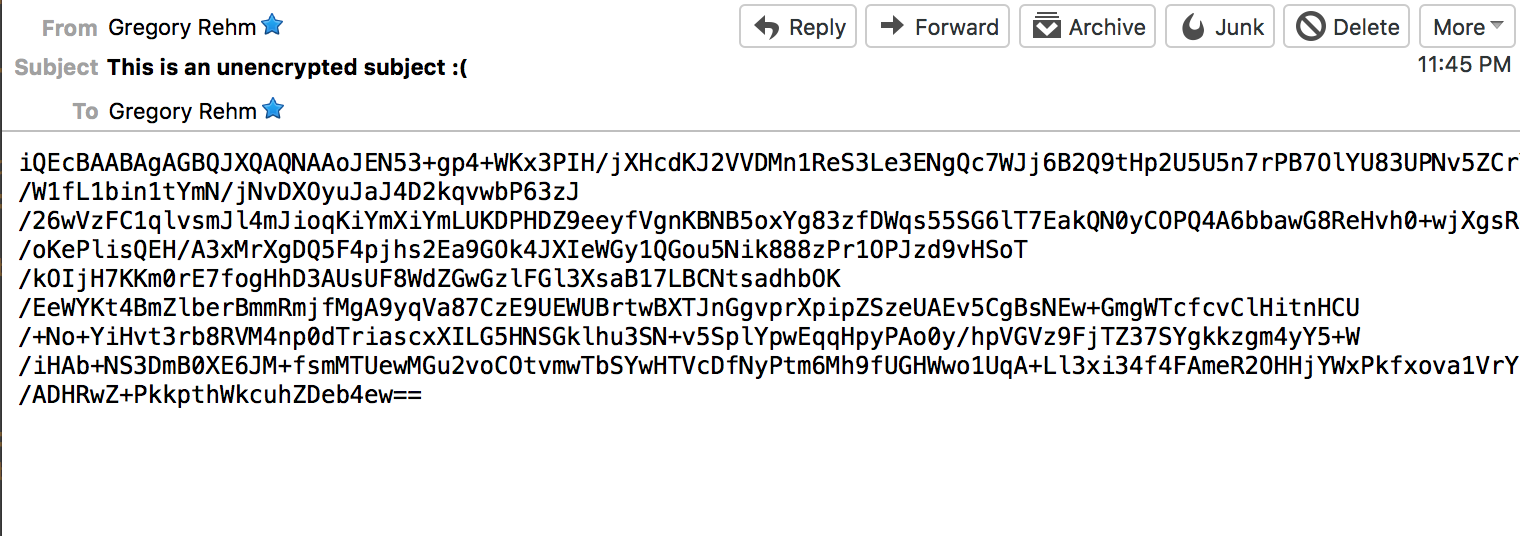
\includegraphics[scale=.5]{encrypted-msg.png}
    \caption{An encrypted message in the mail client}
    \label{fig:Encrypted-client}
\end{figure*}
\begin{figure*}[h]
    \centering
    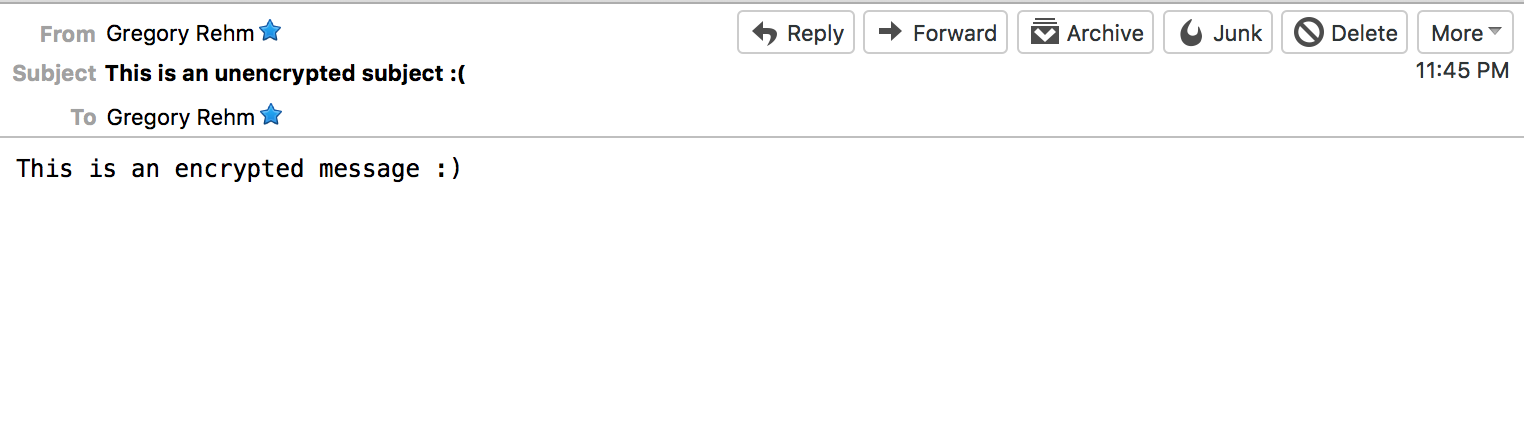
\includegraphics[scale=.5]{decrypted-msg.png}
    \caption{The same message but decrypted after Javascript injection}
    \label{fig:Decrypted-client}
\end{figure*}
\begin{multicols}{2}
\par The mail client plugin is engineered to guarantee that MEG stores no plaintext data for prying eyes to view. Email is stored on the server in encrypted form so the mail provider will have no access to its contents. In order to decrypt a message the MEG plugin looks for a special header attached to all MEG emails and then transmits them to the phone for decryption. When the messages arrive back on the client they are decrypted with the AES-256 symmetric key and then displayed on screen through Javascript injection. However this display is ephemeral and only lasts as long as the user has the message window open. When the user closes the message no decrypted information is stored in a database and the decrypted information is garbage collected. In Figure \ref{fig:Encrypted-client} we can see how the user would initially view their email at rest in the client. In Figure \ref{fig:Decrypted-client} we can see that exact same message after the Javascript injection occurs.
\section{Usability}
Our primary aim was to make MEG as usable as possible to ensure people with little technical training would be able to encrypt their mail. In the MEG system there are two components that users are meant to interact with: the mail client plugin and the mobile app. First we will show how the mobile app's minimal UI makes generating PGP keys as painless as possible for users. We also show that the generation of symmetric key information does not require any technical skill. Then we show how the mail client plugin enables users to use the same mail services they are familiar with to send encrypted mail just by the click of a button.
\subsection{Mobile App Usability}
\par The MEG mobile app is where all PGP encryption, decryption, signing, and key generation actions take place. Fortunately, users need to perform no manual work on their ends to accomplish this task themselves. The app is also designed to be as minimal as possible. First of all, are only four different UI panels that the user can actually navigate to ensuring that we reduce navigation confusion. Second, the app is designed to make the process of generating a PGP key as simple as possible. Below we see that only five pieces of information are needed from the user to generate a PGP public/private key pair: first and last name, phone number, email, and password. After inputting this information the user a PGP public/private key pair will be generated for so they can start using MEG.
\begin{center}
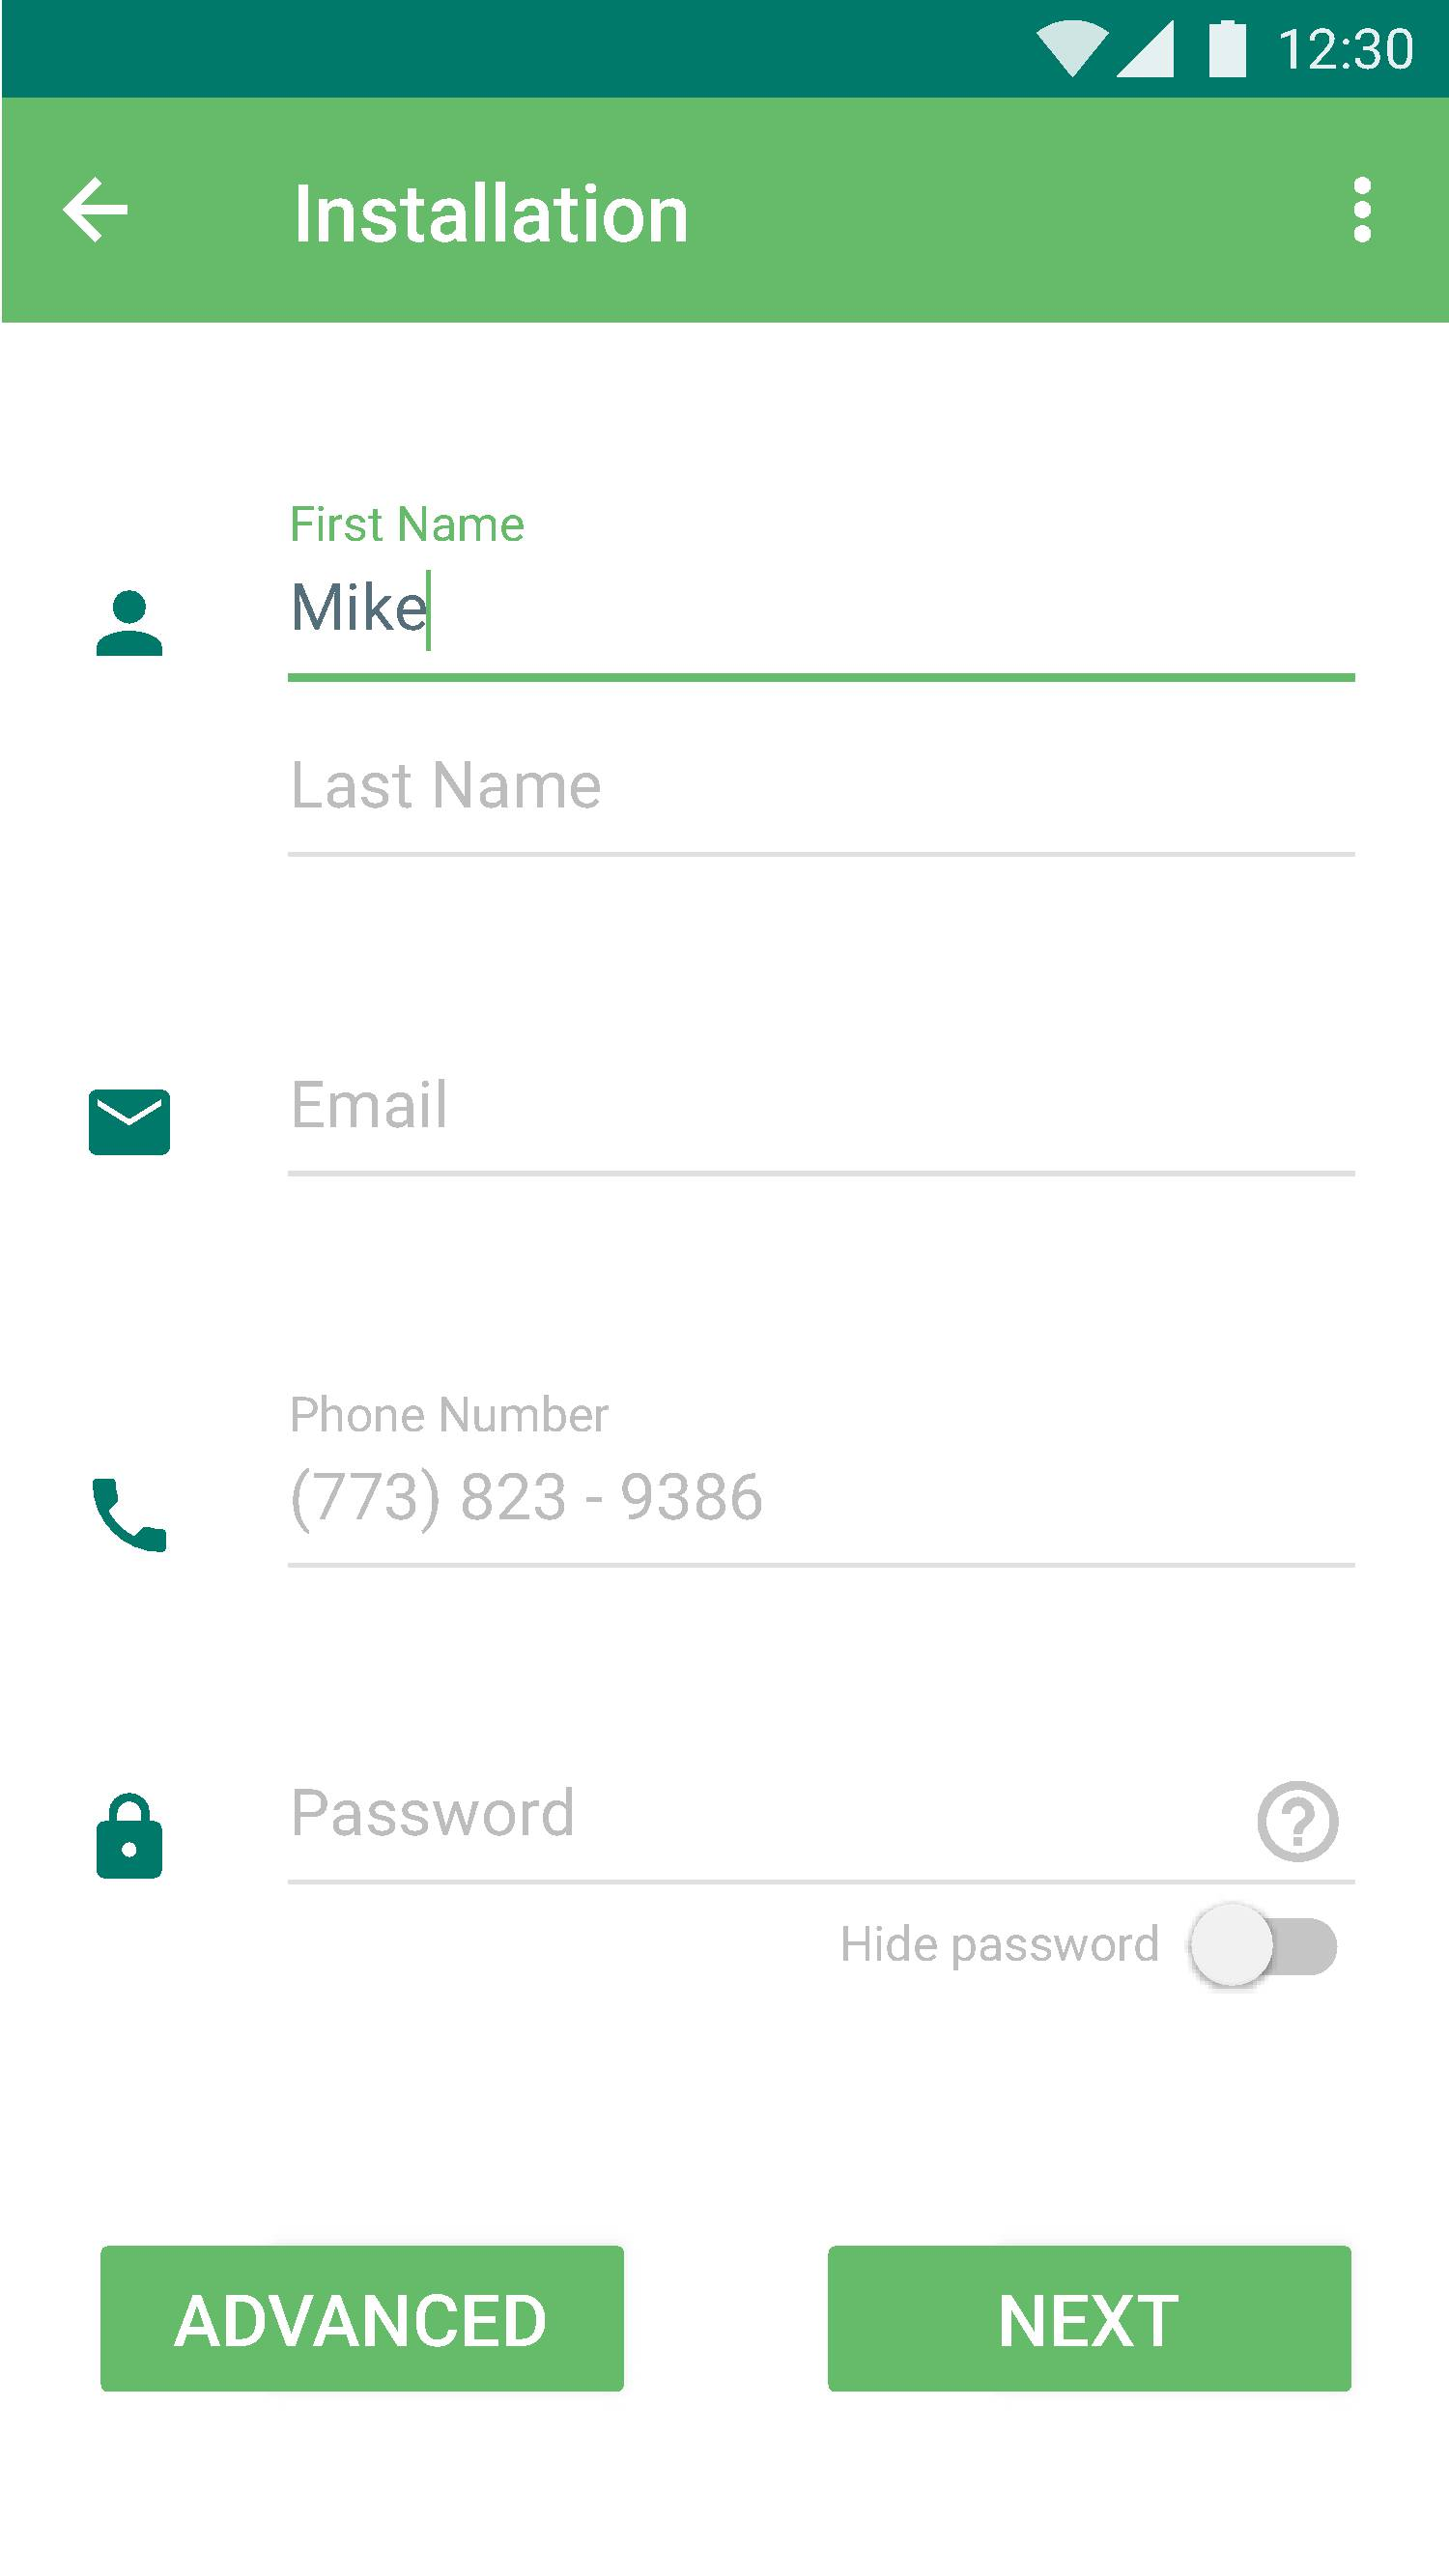
\includegraphics[height=8cm,width=5cm]{installation-page.jpg}
\label{fig:installation}
\end{center}
\par After generating a public/private key pair the MEG app needs to scan a QR code to authenticate a mail client plugin. In security applications QR codes have shown promise. QR codes have even been used for physical access control \cite{qrcode-authentication} and can securely transmit PGP information\cite{qrcode-key-distribution}. In MEG, we use a QR code to transmit AES-256 symmetric key information from the mail client plugin to the mobile app. This way we can transmit private key information without the key ever being transmitted over the network. This symmetric key information is then used to encrypt communications between the mail plugin and the the phone. The symmetric key is generated in the mail client plugin as shown below. After the QR code is scanned the image is removed from the screen ensuring that malicious actors cannot gain access to the symmetric key information. The main advantages of using a QR code to to transmit symmetric key information is that it is both secure and easy to use. Most users are well acquainted with using their mobile devices camera. Furthermore the use of a QR code precludes the necessity of performing additional password input in the mail client ensuring that the user only needs to remember one password when using MEG.
\begin{center}
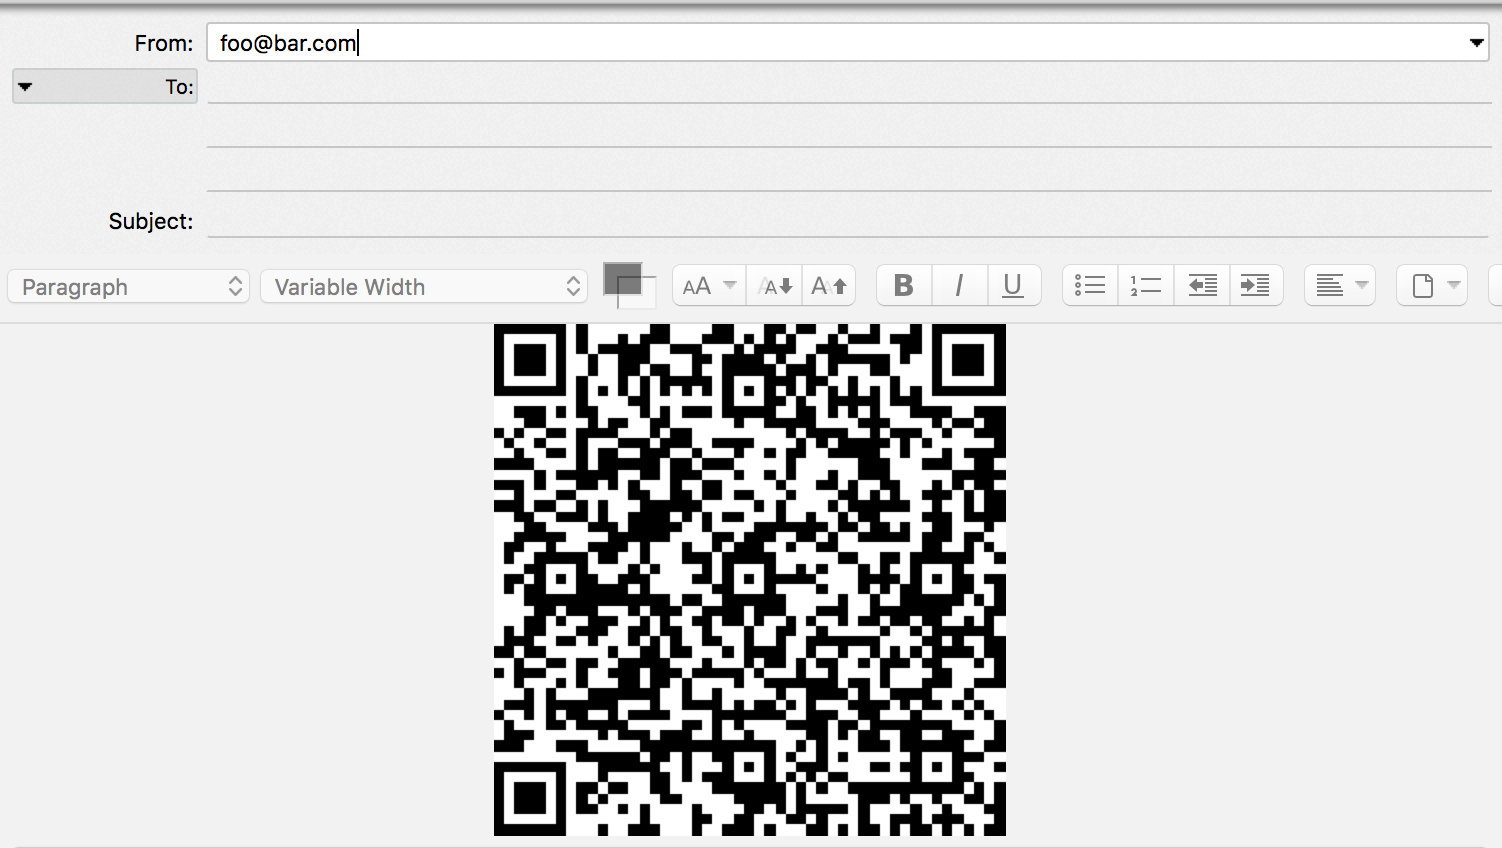
\includegraphics[width=8cm,height=6cm]{qr-code-thunderbird.png}
    %\caption{A QR Code Ready to be Scanned}
\label{fig:qr}
\end{center}
\par A negative of some mail encryption applications is that a user must continually input their password each time they want to send and receive email. This is especially true of server based applications because caching a decrypted private key would mean the service is not end to end encrypted and that the application could access the user's encrypted files. Because all encryption actions occur on a user's phone, and the phone is in physical possession of a user, MEG is able to avoid the user having to re-enter their password each time an email is encrypted or decrypted. Instead, MEG implements private key caching. Upon starting, MEG mobile app users will need to enter their password to unlock their private key. Then the key is cached and is able to be reused as long as the app stays open. This ensures that users can encrypt and decrypt their mail merely by having their phone on and MEG open. If the mobile app is closed by the user or the OS for some reason then the user will need to log back into the mobile app. Ultimately this will be detected if a user attempts to either send or decrypt an email on the client. The client will then alert the user they need to log back into the mobile app to complete their action.
\subsection{Client Usability}
\par While the mobile app performs all PGP actions, the client plugin is where the majority of user interaction will occur in MEG. As such we designed it so that users would have to do as few actions as possible to encrypt their messages.
\par The two main actions a user will need to perform on the mail client are generating a QR code so symmetric key data can be sent to the phone, and sending encrypted mail. The QR code is generated on the first attempt the user makes to send a piece of encrypted mail. Once scanned the QR code is removed from screen through user confirmation the code was scanned successfully. After confirmation users can begin to send encrypted mail.
\end{multicols}
\begin{figure*}[h]
    \centering
    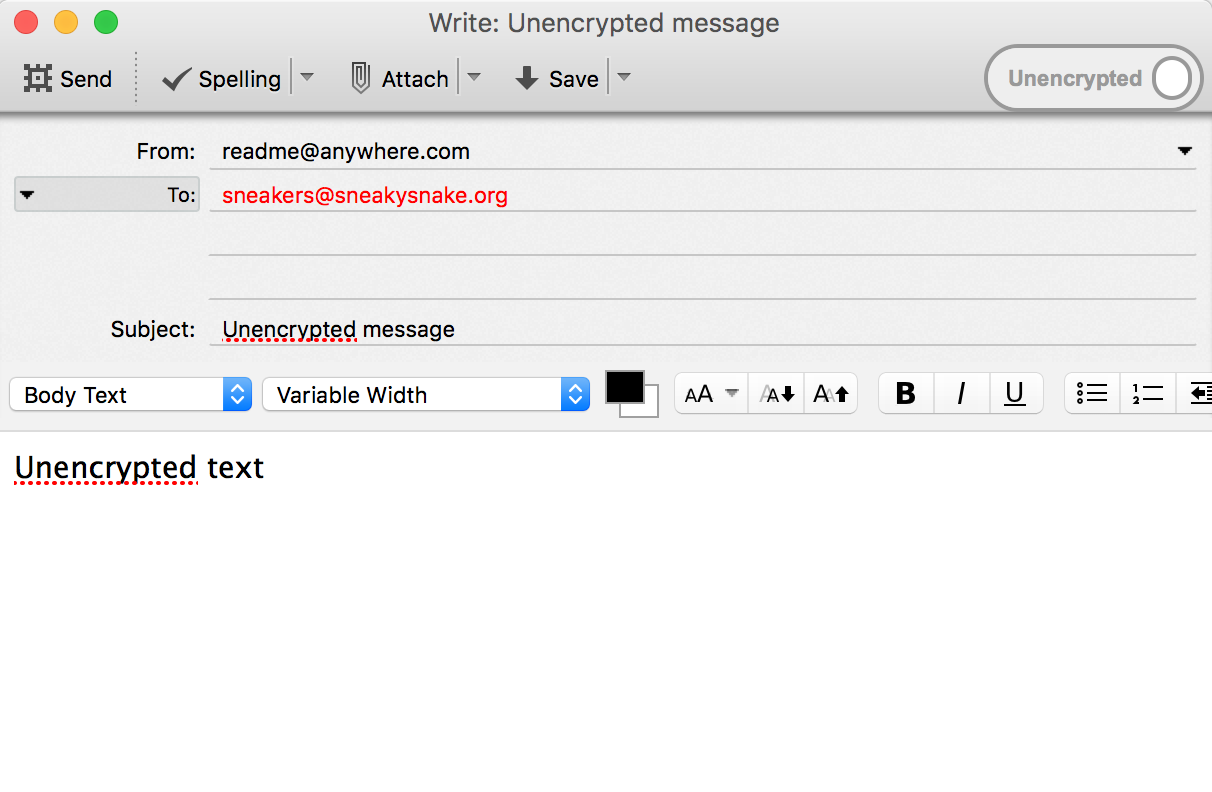
\includegraphics[scale=.5]{unencrypted-client-ui.png}
    \caption{Client UI for sending unencrypted messages}
    \label{fig:unencrypted-ui}
\end{figure*}
\begin{figure*}[h]
    \centering
    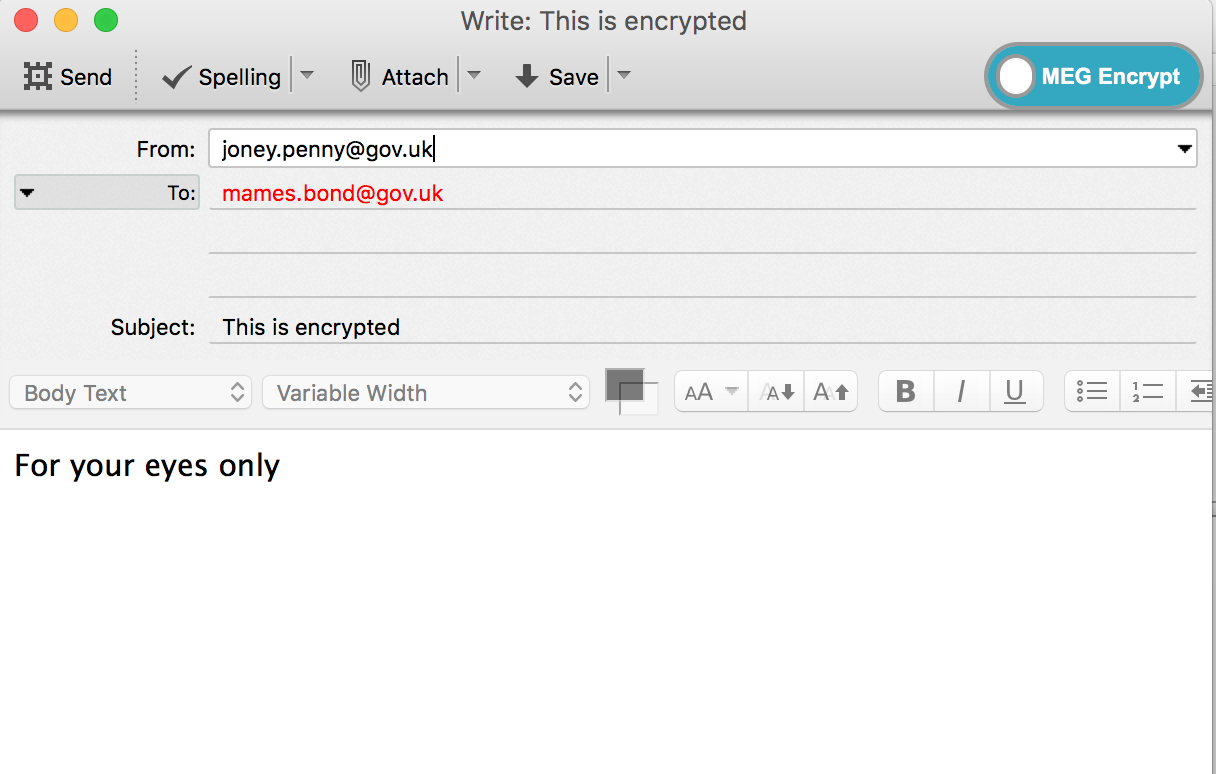
\includegraphics[scale=.5]{encrypted-client-ui.png}
    \caption{Client UI for sending encrypted messages}
    \label{fig:encrypted-ui}
\end{figure*}
\begin{multicols}{2}
\par Encrypted mail is toggled through a checkbox at the top of the mail client. We always give the user the option to have their mail unencrypted in case someone in their network is unable to read their encrypted mail. This is shown in Figure \ref{fig:unencrypted-ui} Encrypting mail is as easy as clicking the encrypt checkbox. We show the implementation in Thunderbird in Figure \ref{fig:encrypted-ui}.
\par Once the user is finished composing his or her mail they only need to click the send button. As a result learning a new flow for sending an encrypted email is not necessary beyond clicking a checkbox. This is a hurdle that Thunderbird by default and some mail plugins like Enigmail introduce to their users \cite{enigmail-handbook}. MEG is able to avoid this problem mainly because PGP is handled automatically on Android but also because of its overall focus on usability.
\par If an encrypted email is attempted to be sent to a user without MEG or some otherwise accessible public key then we will send an email asking the user to sign up for MEG services. This operates in a similar way to the ways that social networks like Facebook became so popular, through electronic word of mouth \cite{trusov2009effects}. This approach will help alleviate the network effect problems associated with encrypted email.
\section{Future Work}
\par We have shown here how MEG offers a secure and accessible application to perform email encryption. Future directions should focus on making the software as usable as possible. The requirement to scan a QR code may be onerous for users so it is possible there are other routes to disseminate symmetric key information from using the server as an origin over HTTPS. It has also been suggested that IPv6 would allow us to eliminate the server altogether as a message router allowing the client plugin to directly communicate with our phone.
\par Currently MEG is in a proof of concept and we hope to make it accessible to as many people as possible in the future. So additional work will need to be done on hardening the system against errors that can occur from network instability or user error. To reach a wider user base we'd like to start work on an iOS app and a Gmail plugin.

\section{Conclusion}
\par MEG is a free, mail client agnostic, encryption application that automates the pain points of email encryption. MEG ensures that users do not have to worry about the details of securing their messages. These characteristics mean that MEG will be both more secure and more accessible than other email encryption schemes. MEG has the benefit of being able to learn from its predecessors. We have the ability to understand where previous schemes such as KCM failed. We also have the benefit of being able to use the ubiquity of smartphones to serve as email gateways. Network effects that prevent ubiquitous encryption can be ameliorated by ensuring MEG is as usable as possible. We believe that the choice between security and usability does not have to be a major tradeoff for users. It is rather just a matter of engineering the correct solution that average people can use. We believe MEG is the best solution for email encryption.

\bibliographystyle{plain}
\bibliography{ecs289m-final-paper.bib}
\end{multicols}
\end{document}
